\chapter{Proportionnalité}\label{ChProportionnalite}

\vspace{5cm}
\begin{acquis}
\begin{itemize}
\item identifier une situation de proportionnalité;
\item calculer le coefficient de proportionnalité d’un tableau;
\item compléter un tableau de proportionnalité en utilisant les relations entre lignes ou entre colonnes;
\item résoudre un problème de proportionnalité.
\end{itemize}
\end{acquis}


\activites

\begin{activite}[Proportionnalité ou pas ?]

\begin{center} 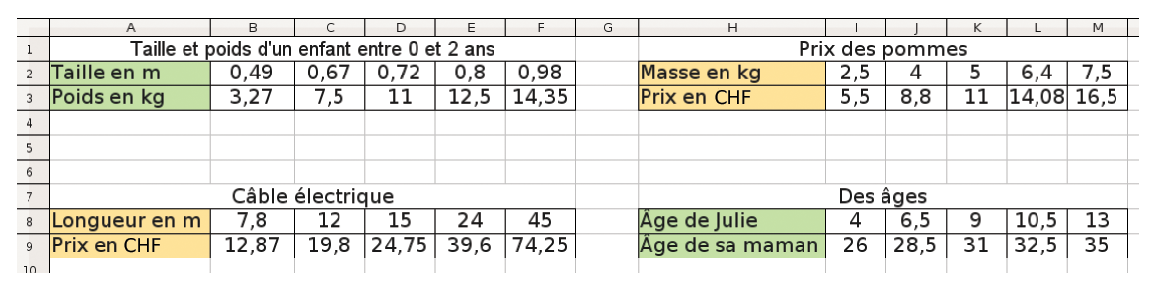
\includegraphics[width=15.8cm]{propor_pas} \end{center}

\begin{enumerate}
 \item Considère séparément chacun des tableaux. Les grandeurs comparées sont-elles \textbf{proportionnelles} ? \label{Propor_acti1}
 \item Note dans ton cahier le résultat de $B3 \div B2$ (tu peux utiliser ta calculatrice), puis le résultat de $C3 \div C2$, puis celui de $D3 \div D2$. Que peux-tu en conclure ?
 \item Fais les mêmes calculs pour les autres situations afin de vérifier tes réponses à la question \ref{Propor_acti1}.
 \item Réponds si possible aux questions suivantes.
 \begin{itemize}
  \item Quel sera le poids de l'enfant lorsqu'il mesurera 1 m ?
  \item Quel est le prix de 8 kg de pommes ?
  \item Quel est le prix de 35 m de câble électrique ?
  \item Quel sera l'âge de la maman lorsque Julie aura 17 ans ?
  \end{itemize}
 \end{enumerate}
 
\end{activite}

%%%%%%%%%%%%%%%%%%%%%%%%%%%%%%%%%%%%%%%%%%%%%%%%%%%%%%%%%%%%%%%%%%%%%%%%%

\begin{activite}[Et pour un ?]

Pour composer un lunch, un traiteur propose des toasts et du punch. Il prépare :
\begin{itemize}
 \item six toasts par personne ;
 \item des saladiers de punch de 5 l qui permettent de servir 40 verres chacun.
 \end{itemize}
 \begin{enumerate}
  \item Combien de toasts devra-t-il préparer pour une réception de 30 personnes ? De 45 personnes ? De 60 personnes ? De 75 personnes ?
  \item Un client lui dit : « 5 l pour 40 verres ? N'est-ce pas de trop petites rations ? » Comment faire pour le rassurer ?
  \item Chaque personne ne se servant qu’une fois, quelle quantité de punch le traiteur devra-t-il préparer pour une réception de 30 personnes ? De 45 personnes ? De 60 personnes ? De 75 personnes ?
  \item À la fin d’une réception, il reste 2 l de punch dans un saladier. Combien de verres le traiteur n’a-t-il pas servis ?
  \item Aide-le à réaliser un tableau avec lequel il pourra calculer le volume de punch à préparer pour un nombre de convives précis.
  \end{enumerate}

\end{activite}

%%%%%%%%%%%%%%%%%%%%%%%%%%%%%%%%%%%%%%%%%%%%%%%%%%%%%%%%%%%%%%%%%%%%%%%%%

\begin{activite}[Cœfficient de proportionnalité]

\begin{partie}[À la boulangerie]
\begin{minipage}[c]{0.68\linewidth}
La boulangère veut préparer une feuille de calcul pour lui permettre de déterminer plus rapidement le prix lors de la vente des croissants. \\[0.5em]
Fais un tableau contenant tous les prix de 2 à 10 croissants.
 \end{minipage} \hfill%
 \begin{minipage}[c]{0.28\linewidth}
  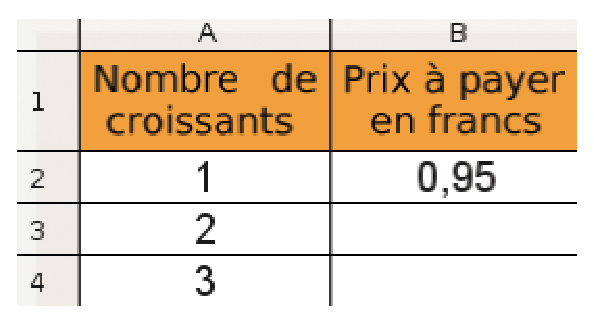
\includegraphics[width=4.2cm]{prix_croissant}
  \end{minipage} \\
\end{partie}

\begin{partie}[Comparaison de prix]
\begin{minipage}[c]{0.68\linewidth}
\begin{enumerate}
 \item À la station Seso, Rachid a acheté 43 l d'essence et a payé 41,71 CHF. Reproduis le tableau et détermine le prix que paiera Julia qui a mis 37 l d'essence dans son réservoir, sachant que le prix à payer est proportionnel au nombre de litres d'essence.
 \item Bruno, lui, a fait le plein de 48 l d'essence à la station Motal et a payé 44,64 CHF. À l'aide d'un tableau, réponds à la question suivante : Bruno aurait‑il dû aller à la même station que Rachid ?
 \end{enumerate}
 \end{minipage} \hfill%
 \begin{minipage}[c]{0.28\linewidth}
  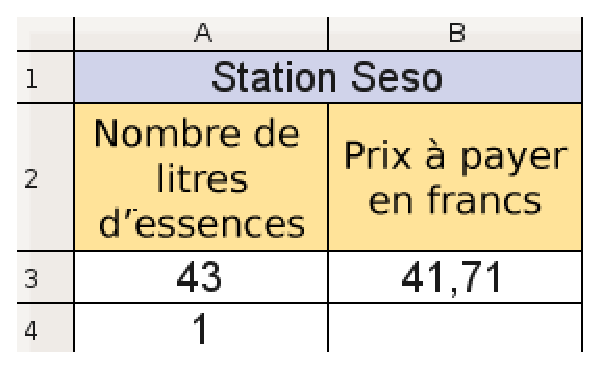
\includegraphics[width=4.2cm]{prix_essence}
  \end{minipage} \\
\end{partie}

\end{activite}

%%%%%%%%%%%%%%%%%%%%%%%%%%%%%%%%%%%%%%%%%%%%%%%%%%%%%%%%%%%%%%%%%%%%%%%%%

\begin{activite}[Premiers calculs]

Dans une jardinerie, la pancarte ci-dessous indique le nombre de sacs de graines à utiliser en fonction de la surface du terrain à ensemencer. \\[0.5em]

\begin{minipage}[c]{0.48\linewidth}
\begin{center} Terrain de 375 m\up{2} \end{center}
\vspace{0.3cm}
\begin{center} 
\includegraphics[width=2.2cm]{3sacs_gazon} \end{center}
 \end{minipage} \hfill%
 \begin{minipage}[c]{0.48\linewidth}
\begin{center} Terrain de 500 m\up{2} \end{center}
\vspace{0.3cm}
\begin{center} 
\includegraphics[width=2.2cm]{4sacs_gazon} \end{center}
  \end{minipage} \\

\begin{enumerate}  
 \item À l’aide de cette illustration, réponds aux questions suivantes :
 \begin{itemize}
  \item Quelle surface pourra ensemencer Jean-Paul avec 7 sacs ?
  \item Quelle surface pourra ensemencer Emmanuel avec 6 sacs ?
  \item De combien de sacs aura besoin Rachid pour réaliser une pelouse de 1\,500 m\up{2} ?
  \item Quelle surface pourra ensemencer Léonard avec 19 sacs ?
  \item Quelle surface pourra ensemencer Fatima avec 28 sacs ?
  \item De combien de sacs aura besoin Steeve pour réaliser une pelouse de 3\,875 m\up{2} ?
  \item Quelle surface pourra ensemencer Sonda avec 21 sacs ?
  \end{itemize}
 \item Trouve un moyen simple de présentation pour synthétiser ces questions et ces réponses.
 \item Propose plusieurs méthodes pour déterminer quelle surface de gazon on peut recouvrir avec un seul sac.
\end{enumerate}

\end{activite}

%%%%%%%%%%%%%%%%%%%%%%%%%%%%%%%%%%%%%%%%%%%%%%%%%%%%%%%%%%%%%%%%%%%%%%%%%

\begin{activite}[Recette de cuisine]

\begin{partie}
Pour faire un gâteau pour six personnes, il faut 150 g de sucre :
\begin{enumerate}
 \item Manon souhaite faire un gâteau deux fois moins gros. Quelle quantité de sucre doit‑elle utiliser ?
 \item Marine doit faire ce gâteau pour 9 personnes. Propose plusieurs façons de trouver la masse de sucre qu'elle doit utiliser.
 \item Sabrina dispose de 200 g de sucre. Détermine de plusieurs façons pour combien de personnes sera le gâteau.
 \end{enumerate}
\end{partie}

\begin{partie}
Les masses de farine et de sucre sont proportionnelles. Reproduis le tableau de proportionnalité et complète‑le le plus astucieusement possible : \\[0.5em]
\begin{center}
 \begin{tabularx}{0.7\linewidth}{|c|X|X|X|X|X|X|}
 \hline
\rowcolor{H3} Masse de sucre en g & 50 & 130 & 100 & 180 & 230 & 115 \\\hline
\rowcolor{F3} Masse de farine en g & 65 & 169 & & & & \\\hline
 \end{tabularx}
 \end{center}
\end{partie}

\end{activite}

%%%%%%%%%%%%%%%%%%%%%%%%%%%%%%%%%%%%%%%%%%%%%%%%%%%%%%%%%%%%%%%%%%%%%%%%%




\cours
%\section{Une section}

% remarque : pour qu'un mot se retrouve dans le lexique : \MotDefinition{asymptote horizontale}{} 

\begin{aconnaitre}
Deux grandeurs sont \textbf{proportionnelles} lorsque l’une s’obtient en multipliant (ou en divisant) l’autre par un même nombre non nul.

Ce coefficient multiplicateur est un \MotDefinition{coefficient de proportionnalité}{}.
\end{aconnaitre}

\begin{methode*1}[Trouver le coefficient de proportionnalité]

 \begin{exemple*1}
Le carburant pour un motoculteur est un mélange de super et d’huile où les doses d’huile et d’essence sont proportionnelles : il faut 2 doses d’huile pour 3 doses de super. Détermine le coefficient de proportionnalité qui permet d’obtenir la dose de super en fonction de la dose d’huile.
\begin{center} 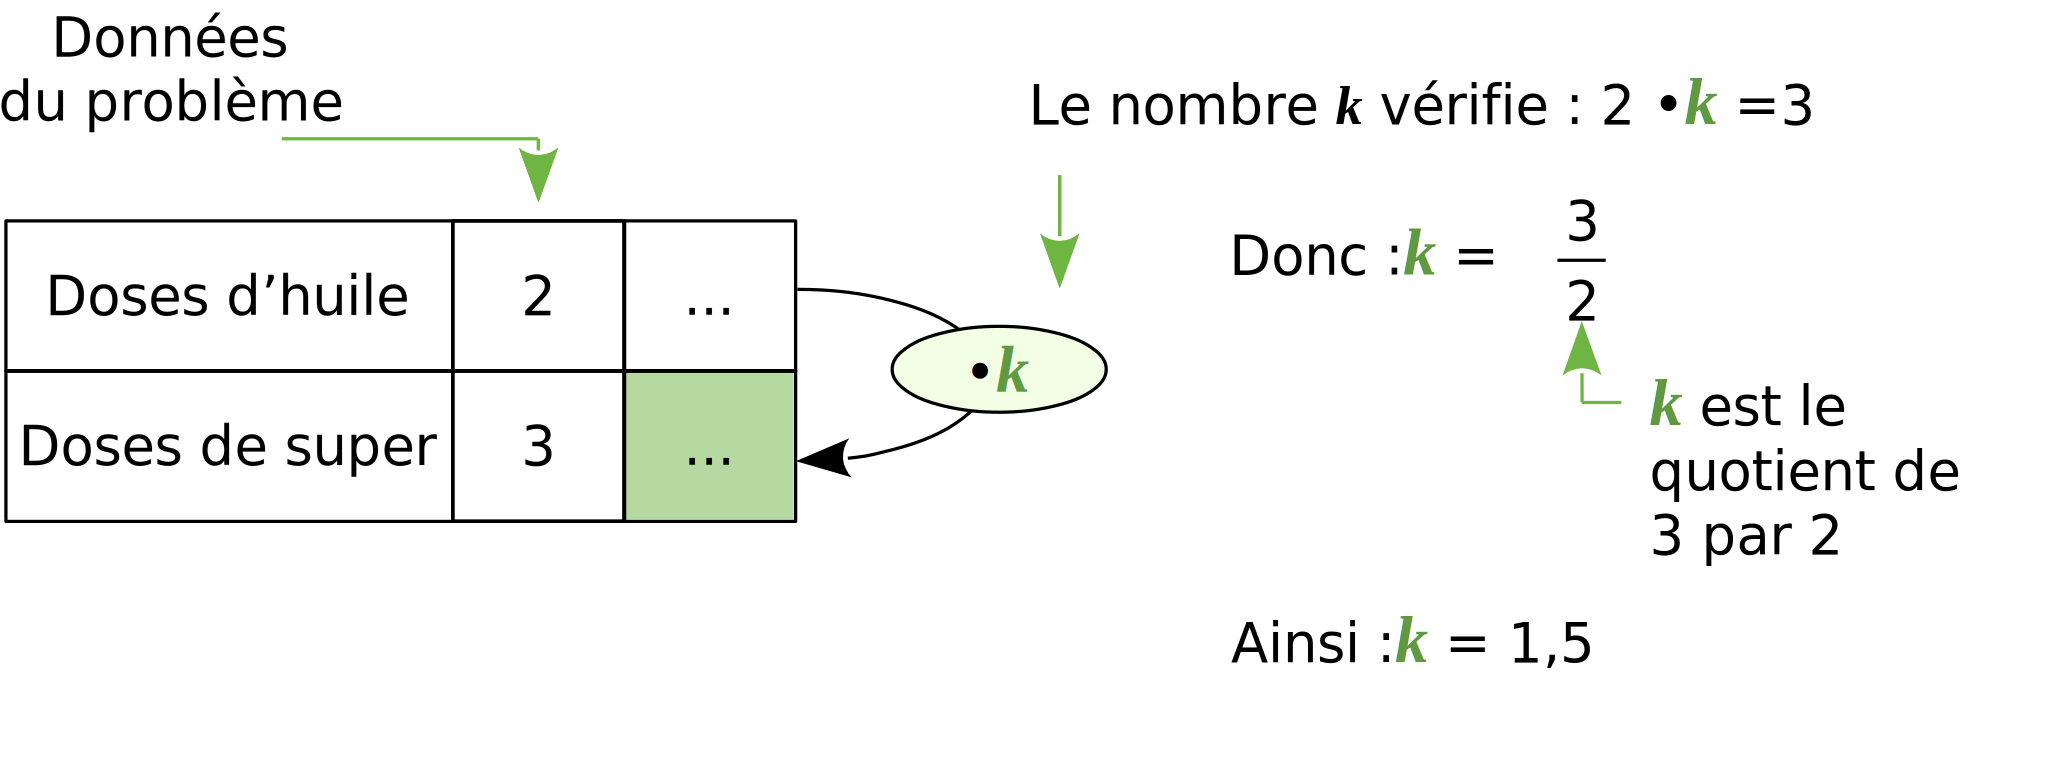
\includegraphics[width=12cm]{probleme_propor1} \end{center}
Le coefficient de proportionnalité qui permet d'obtenir la dose de super en fonction de la dose d'huile est 1,5.
 \end{exemple*1}

 \begin{remarque}
Soit $\textbf{\textcolor{C2}{h}}$ le coefficient de proportionnalité qui permet d'obtenir la dose d’huile en fonction de la dose de super :
\begin{center} 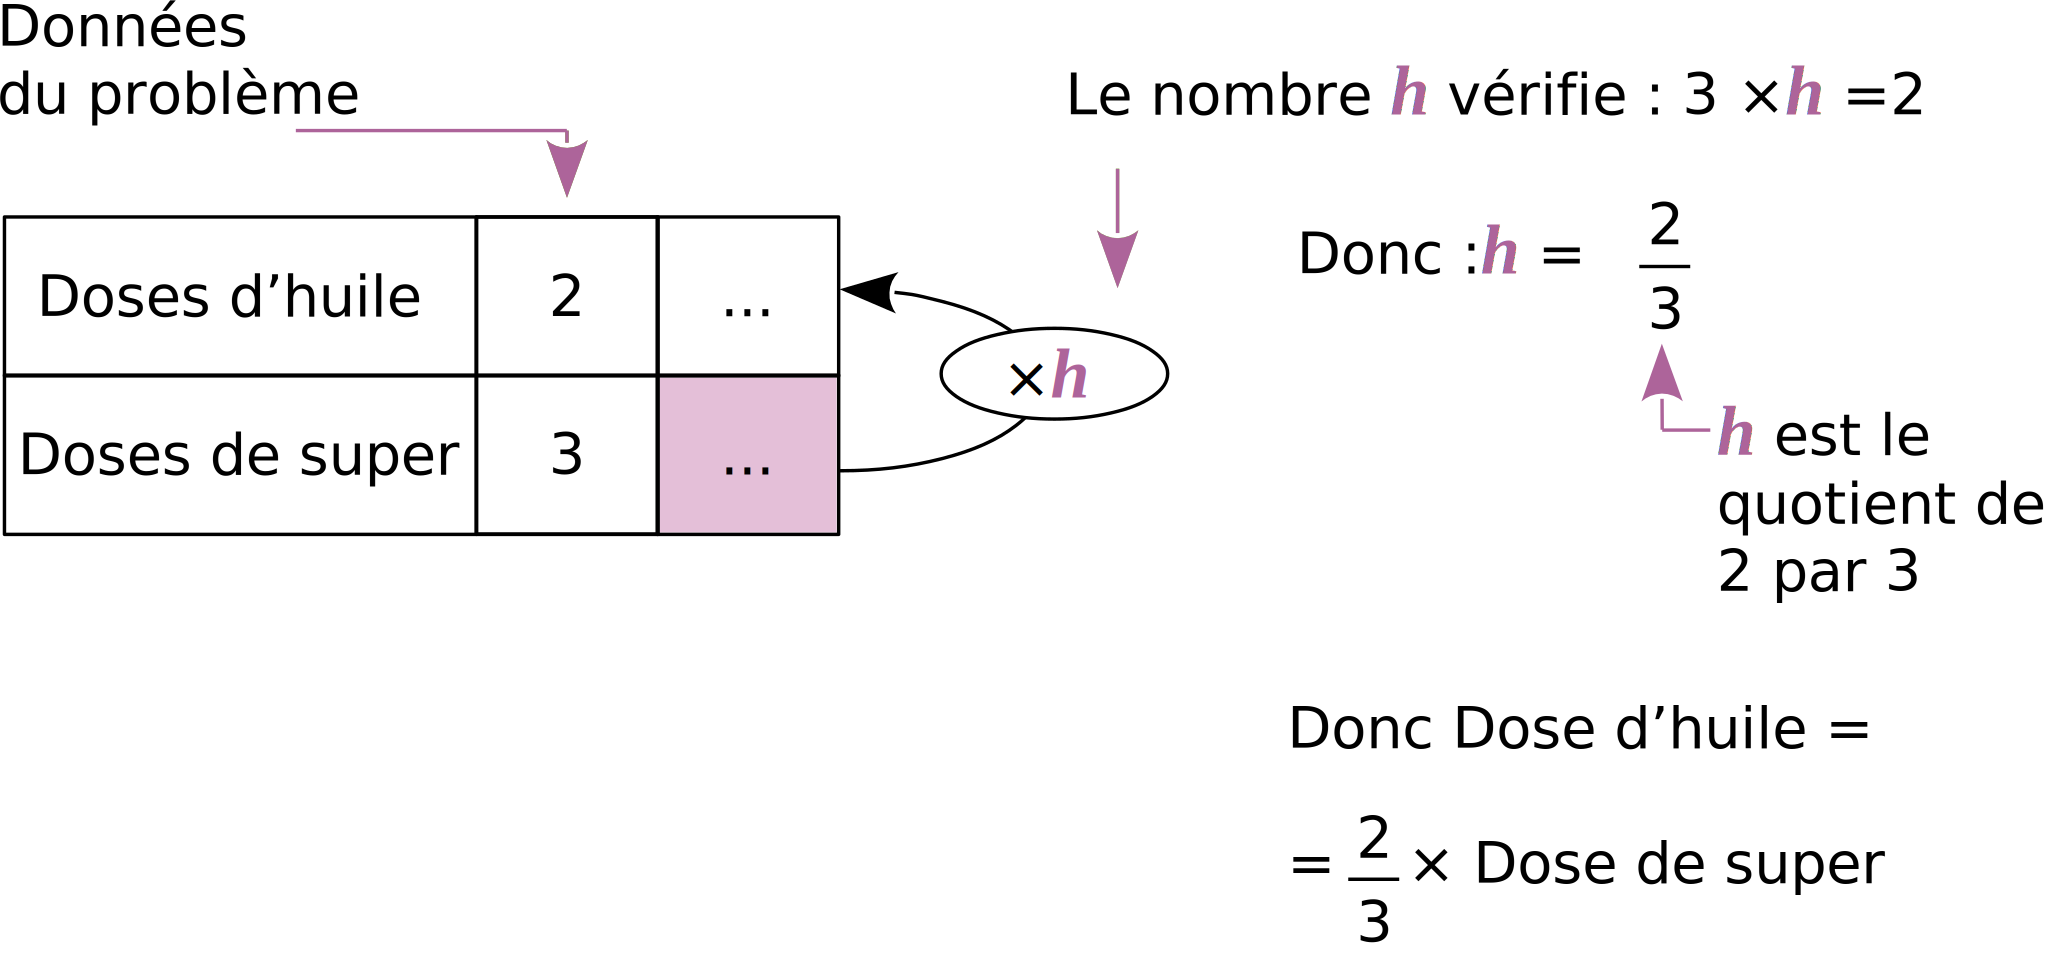
\includegraphics[width=12cm]{probleme_propor2} \end{center}
 \end{remarque}

 \exercice  
Un magasin vend 2 kg de pommes pour 5 CHF. Par quel nombre faut-il multiplier le nombre de kg de pommes pour obtenir celui du prix ?
%\correction

 \end{methode*1}
 
 %%%%%%%%%%%%%%%%%%%%%%%%%%%%%%%%%%%%%%%%%%%%%%%%%%%%%%%%%%%%%%%%%%%%%%%%
 
 \begin{aconnaitre}
Pour vérifier si deux grandeurs sont \MotDefinition{proportionnelles}{}, on doit s’assurer qu’elles évoluent toutes les deux dans les mêmes proportions.
\end{aconnaitre}

\begin{methode*1}[Identifier une situation de proportionnalité]

 \begin{exemple*1}
Les tarifs des remontées mécaniques d’une station de ski sont les suivants : 50 CHF la journée, 90 CHF les deux jours et 240 CHF les 6 jours. Le prix à payer est-il proportionnel à la durée ? \\[1em]
Si le prix à payer était proportionnel à la durée, en payant 50 CHF la journée, on devrait payer le double pour deux jours, soit 100 CHF et 6 fois plus pour six jours, soit 300 CHF. \\[0.5em]
Comme ce n'est pas le cas, le prix à payer n'est pas proportionnel à la durée. 
 \end{exemple*1}

 \exercice  
Un commerçant vend ses croissants à 0,65 CHF l’unité ou à 5,00 CHF le paquet de 10. Cette situation ne relève pas d’une situation de proportionnalité. Explique pourquoi.
%\correction

 \end{methode*1}
 
 %%%%%%%%%%%%%%%%%%%%%%%%%%%%%%%%%%%%%%%%%%%%%%%%%%%%%%%%%%%%%%%%%%%%%%%%

\begin{methode*1}[Utiliser les propriétés de la proportionnalité]

 \begin{exemple*1}
Complète le tableau de proportionnalité suivant :
\begin{center}
\begin{tabularx}{0.8\linewidth}{|c|*{6}{>{\centering\arraybackslash}X|}}
\hline
\cellcolor{C4} Masse de pommes (en kg) & 16 & 8 & 2 & & 24 \\ \hline
\cellcolor{C4} Prix (en CHF) & & 7,8 & & 78 &  \\ \hline
  \end{tabularx}
 \end{center}
\begin{center} 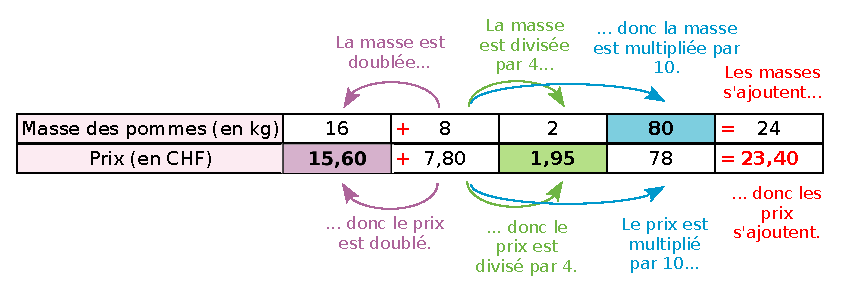
\includegraphics[width=12.5cm]{prix_pommes} \end{center}
 \end{exemple*1}


 \exercice  
La voiture de Marie consomme 4,5 l d'essence sur 100 km :
\begin{enumerate}
 \item Quelle sera sa consommation si elle parcourt 150 km ? 250 km ? 1 250 km ?
 \item La voiture de Marie a consommé 13,5 l d'essence. Quelle distance a‑t‑elle parcourue ? Quelle distance peut-elle parcourir avec 135 l d'essence ?
 \end{enumerate}
%\correction

 \end{methode*1}
 
 %%%%%%%%%%%%%%%%%%%%%%%%%%%%%%%%%%%%%%%%%%%%%%%%%%%%%%%%%%%%%%%%%%%%%%%%


\begin{methode*1}[Calculer avec un cœfficient de proportionnalité]

 \begin{exemple*1}
Lucie paye 100 CHF pour acheter 20 clés. Quelle est le nombre de clés qu'elle peut acheter pour 55 CHF ? Et pour 30 CHF ? Si elle désire acheter 126 clés, Combien devra-t-elle payer ? \\[1em]
Le nombre de clés est proportionnel au prix. \\[0.5em]
\begin{minipage}[c]{0.08\linewidth}
 
\includegraphics[width=1.1cm]{mult_02}
 \end{minipage} \hfill%
 \begin{minipage}[c]{0.8\linewidth}
\begin{tabularx}{\linewidth}{|c|*{4}{>{\centering\arraybackslash}X|}}
\hline
\cellcolor{C4} Coût (en CHF) & 100 & 55 & 30 & \textcolor{B2}{\textbf{630}} \\\hline
\cellcolor{C4} Nombre de clés & 20 &  \textcolor{A2}{\textbf{11}} &  \textcolor{A2}{\textbf{6}} & 126 \\\hline
  \end{tabularx}
  \end{minipage} \hfill%
  \begin{minipage}[c]{0.08\linewidth}
   
\includegraphics[width=1.1cm]{div_02}
   \end{minipage} \\ 
\begin{itemize}
 \item On calcule le coefficient \textbf{de proportionnalité} : $20 : 100 =$ \textcolor{A2}{\textbf{0,2}}.
 \item Pour trouver les nombres de la 2\up{e} ligne du tableau, on multiplie les nombres de la 1\up{re} ligne par le coefficient de proportionnalité. Pour trouver les nombres de la 1\up{re} ligne du tableau, on divise les nombres de la 2\up{e} ligne par le coefficient de proportionnalité.
  \end{itemize}
 \end{exemple*1}


 \exercice
Complète le tableau de proportionnalité suivant :
\begin{center}
\begin{tabularx}{0.9\linewidth}{|c|*{5}{>{\centering\arraybackslash}X|}}
\hline
\cellcolor{C4} Nombre de personnes & 7 & 13 & 5 & & \\\hline
\cellcolor{C4} Prix payé pour entrer au cinéma (en CHF)
 & 45,50 & & & 65 & 71,50 \\\hline
  \end{tabularx}
 \end{center}
%\correction

 \exercice
Un skipper doit acheter plusieurs bouts de cordage. Il choisit un cordage à 17,50 CHF les cinq mètres. Combien coûte un bout de 15 m ? De 3,5 m ? De 23 m ? Quelle longueur obtient-il avec 87,50 CHF ?
%\correction

 \end{methode*1}
 
 %%%%%%%%%%%%%%%%%%%%%%%%%%%%%%%%%%%%%%%%%%%%%%%%%%%%%%%%%%%%%%%%%%%%%%%%
 
 
%%%%%%%%%%%%%%%%%%%%%%%%%%%%%%%%%%%
%%%%%%%%%%%%%%%%%%%%%%%%%%%%%%%%%%%
%MiseEnPage
%%%%%%%%%%%%%%%%%%%%%%%%%%%%%%%%%%%
\newpage
%%%%%%%%%%%%%%%%%%%%%%%%%%%%%%%%%%%
%%%%%%%%%%%%%%%%%%%%%%%%%%%%%%%%%%%
 
\begin{aconnaitre}
Un tableau de nombres relève d’une situation de proportionnalité si un même coefficient (non nul) multiplicateur s’applique dans \textbf{tout} le tableau. On parle alors de \MotDefinition{coefficient de proportionnalité}{}.
\end{aconnaitre}

\begin{methode*1}[Reconnaître un tableau de proportionnalité]

 \begin{exemple*1}
Ces tableaux de nombre sont-ils des tableaux de proportionnalité ? \\[0.7em]
\begin{minipage}[c]{0.48\linewidth}
\textbf{1)} \\[0.5em]
 \renewcommand*\tabularxcolumn[1]{>{\centering\arraybackslash}m{#1}}
  \begin{ttableau}{\linewidth}{5}
   \hline
   5 & 8 & 14 & 19 & 24 \\\hline
   12 & 19,2 & 33,6 & 45,6 & 57,6 \\\hline
  \end{ttableau}
 \end{minipage} \hfill%
 \begin{minipage}[c]{0.48\linewidth}
  \textbf{2)} \\[0.5em]
  \renewcommand*\tabularxcolumn[1]{>{\centering\arraybackslash}m{#1}}
  \begin{ttableau}{\linewidth}{5}
   \hline
   12 & 18 & 32 & 27 & 54 \\\hline
   8 & 12 & 20 & 18 & 36 \\\hline
  \end{ttableau}
 \end{minipage} \\
 
 \begin{enumerate}
 \item $\dfrac{12}{5} =$ \textbf{2,4} donc 2,4 est un coefficient de proportionnalité potentiel et on vérifie qu'il convient pour les autres valeurs :
\begin{center}
 \begin{tabular}{rr}
$8 \cdot \text{\textbf{2,4}} = 19,2$ & $14 \cdot \text{\textbf{2,4}} = 33,6$ \\
$19 \cdot \text{\textbf{2,4}} = 45,6$ & $24 \cdot \text{\textbf{2,4}} = 57,6$ \\
  \end{tabular}
 \end{center}
On obtient bien les valeurs du tableau, c’est un tableau de proportionnalité.
 \item On calcule les quotients : \\[0.5em]
 \begin{center} $\dfrac{12}{8} = 1,5$ \qquad $\dfrac{18}{12} = 1,5$ \qquad $\dfrac{\text{\textbf{32}}}{\text{\textbf{20}}} = 1,6$ \end{center}
\vspace{0.5cm}
On a trouvé un quotient différent des deux précédents, il est inutile de calculer les suivants. Ce n’est donc pas un tableau de proportionnalité.
  \end{enumerate}
 \end{exemple*1}

 \exercice  
Ces tableaux sont-ils des tableaux de proportionnalité ?
\begin{minipage}[c]{0.48\linewidth}
\textbf{1)} \\[0.5em]
 \renewcommand*\tabularxcolumn[1]{>{\centering\arraybackslash}m{#1}}
  \begin{ttableau}{\linewidth}{4}
   \hline
   3,4 & 7,5 & 9 & 11,6 \\\hline
   6,8 & 15 & 18,9 & 23,2 \\\hline
  \end{ttableau}
 \end{minipage} \hfill%
 \begin{minipage}[c]{0.48\linewidth}
  \textbf{2)} \\[0.5em]
  \renewcommand*\tabularxcolumn[1]{>{\centering\arraybackslash}m{#1}}
  \begin{ttableau}{\linewidth}{4}
   \hline
   7 & 11 & 18 & 24 \\\hline
   9,1 & 12,1 & 19,8 & 26,4 \\\hline
  \end{ttableau}
 \end{minipage} \\
%\correction

 \end{methode*1}
 
 %%%%%%%%%%%%%%%%%%%%%%%%%%%%%%%%%%%%%%%%%%%%%%%%%%%%%%%%%%%%%%%%%%%%%%%%


\exercicesbase
\begin{colonne*exercice}

\serie{Proportionnalité ou pas ?}

\begin{exercice}[Chez le primeur]
\begin{enumerate}
 \item Pour les pommes, il est affiché « 2,85 CHF le kg ». Le prix des pommes est‑il proportionnel à la quantité achetée ? Justifie.
 \item Pour les pamplemousses, il est affiché « 1,20 CHF l'unité, 2 CHF les deux ». Le prix des pamplemousses est‑il proportionnel à la quantité achetée ? Pourquoi ?
 \end{enumerate}
\end{exercice}


\begin{exercice}
Pour chaque tableau, indique si les deux grandeurs considérées sont proportionnelles ou non. Justifie tes réponses.
\begin{enumerate}
 \item \emph{Prix des stylos} :
 \vspace{0.3cm}
 \begin{center}
  \begin{tabularx}{\linewidth}{|c|*{3}{>{\centering\arraybackslash}X|}}
  \hline
 \rowcolor{H3} Nombre de stylos & 3 & 5 & 7 \\\hline
 \rowcolor{J3} Prix payé (en CHF) & 12 & 20 & 28 \\\hline
 \end{tabularx}
\end{center}
 \vspace{0.3cm}
 \item \emph{Prix des photos de classe} :
 \vspace{0.3cm}
  \begin{center}
  \begin{tabularx}{\linewidth}{|c|*{3}{>{\centering\arraybackslash}X|}}
  \hline
 \rowcolor{H3} Nombre de photos & 2 & 5 & 10 \\\hline
 \rowcolor{J3} Prix payé (en CHF) & 16 & 40 & 60 \\\hline
 \end{tabularx}
\end{center}
 \vspace{0.3cm}
 \item \emph{Quantité de béton nécessaire à la fabrication de ciment} :
 \vspace{0.3cm}
 \begin{center}
  \begin{tabularx}{\linewidth}{|c|*{3}{>{\centering\arraybackslash}X|}}
  \hline
 \rowcolor{H3} Quantité de béton (en m\up{3}) & 1 & 4 & 6 \\\hline
 \rowcolor{J3} Quantité de ciment (en kg) & 350 & 1\,400 & 2\,100 \\\hline
 \end{tabularx}
\end{center}
 \vspace{0.3cm}
 \item \emph{Distance parcourue en fonction de la durée du parcours} :
 \vspace{0.3cm}
 \begin{center}
  \begin{tabularx}{\linewidth}{|c|*{3}{>{\centering\arraybackslash}X|}}
  \hline
 \rowcolor{H3} Durée (en min) & 7 & 6 & 4 \\\hline
 \rowcolor{J3} Distance (en km) & 12,25 & 10,5 & 7 \\\hline
 \end{tabularx}
\end{center}
 \end{enumerate}
\end{exercice}


\begin{exercice}
Les tableaux suivants sont‑ils des tableaux de proportionnalité ? Justifie.

\begin{minipage}[c]{0.48\linewidth}
\textbf{1)}
\begin{center}
 \renewcommand*\tabularxcolumn[1]{>{\centering\arraybackslash}m{#1}}
 \begin{ttableau}{\linewidth}{3}
 \hline
 \rowcolor{J1} 2 & 3 & 7 \\\hline
 \rowcolor{H1} 8 & 12 & 28 \\\hline
 \end{ttableau}
\end{center}
\end{minipage} \hfill%
 \begin{minipage}[c]{0.48\linewidth}
\textbf{3)} 
\begin{center}
 \renewcommand*\tabularxcolumn[1]{>{\centering\arraybackslash}m{#1}}
 \begin{ttableau}{\linewidth}{3}
 \hline
 \rowcolor{J1} 2 & 4 & 5 \\\hline
 \rowcolor{H1} 7 & 14 & 17,5 \\\hline
 \end{ttableau}
\end{center} 
\end{minipage} \\

 \begin{minipage}[c]{0.48\linewidth}
\textbf{2)}
\begin{center}
 \renewcommand*\tabularxcolumn[1]{>{\centering\arraybackslash}m{#1}}
 \begin{ttableau}{\linewidth}{3}
 \hline
 \rowcolor{J1} 2 & 3 & 4 \\\hline
 \rowcolor{H1} 15 & 21 & 28 \\\hline
 \end{ttableau}
\end{center}
\end{minipage} \hfill%
 \begin{minipage}[c]{0.48\linewidth}
\textbf{4)} 
\begin{center}
 \renewcommand*\tabularxcolumn[1]{>{\centering\arraybackslash}m{#1}}
 \begin{ttableau}{\linewidth}{3}
 \hline
 \rowcolor{J1} 2 & 5 & 9 \\\hline
 \rowcolor{H1} 3,2 & 8 & 15 \\\hline
 \end{ttableau}
\end{center} 
\end{minipage} \\

\end{exercice}


\begin{exercice}
Sur une attraction d'une fête foraine, on peut lire : « 4 tickets pour 10 CHF, 10 tickets pour 18 CHF ». Les prix sont‑ils proportionnels au nombre de tickets achetés ? Justifie ta réponse.
\end{exercice}


\begin{exercice}[La taille d'un enfant]
À 2 ans, un enfant mesurait 88 cm. à 3 ans, il mesurait 102 cm. La taille de cet enfant est‑elle proportionnelle à son âge ? Justifie ta réponse.
\end{exercice}


\begin{exercice}[Des rectangles]
\begin{center} 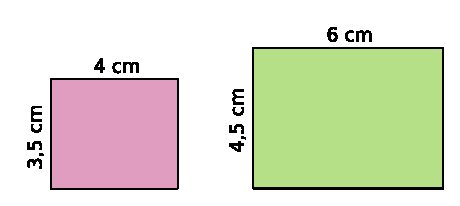
\includegraphics[width=7.4cm]{rectangles_rv} \end{center}
Les dimensions du premier rectangle sont‑elles proportionnelles aux dimensions du second rectangle ? Justifie ta réponse.
\end{exercice}


\begin{exercice}[Carré]
\begin{enumerate}
 \item Calcule le périmètre d'un carré de côté 3 cm.
 \item Le périmètre d'un carré est‑il proportionnel à la longueur du côté de ce carré ? Explique.
 \end{enumerate}
\end{exercice}


\begin{exercice}
Un cinéma propose les tarifs suivants :
 \begin{center}
  \begin{tabularx}{\linewidth}{|c|*{3}{>{\centering\arraybackslash}X|}}
  \hline
  Nombre de séances & 1 & 4 & 12 \\\hline
  Prix à payer (en CHF) & 12 & 48 & 135 \\\hline
 \end{tabularx}
\end{center}
Le prix est-il proportionnel au nombre de séances ?
\end{exercice}

%%%%%%%%%%%%%%%%%%%%%%%%%%%%%%%%%%%%%%%%%%%%%%%%%%%%%%%%%%%%%%%%%%%%%%%%

\serie{Compléter un tableau de proportionnalité}

\begin{exercice}
Complète les tableaux de proportionnalité :
\begin{enumerate}
 \item 
 
 \begin{minipage}[c]{0.18\linewidth}
 
\includegraphics[width=1.9cm]{bulle_mult6} 
  \end{minipage} \hfill
   \begin{minipage}[c]{0.76\linewidth}
   \begin{center}
 \renewcommand*\tabularxcolumn[1]{>{\centering\arraybackslash}m{#1}}
 \begin{ttableau}{\linewidth}{4}
 \hline
 \rowcolor{G2} 3 & 4 & 7,5 & \\\hline
 \rowcolor{D2} & & & 54 \\\hline
 \end{ttableau}
\end{center}
    \end{minipage} \\
\vspace{0.5cm}
 \item 
 
 \begin{minipage}[c]{0.18\linewidth}
 
\includegraphics[width=1.9cm]{bulle_mult12} 
  \end{minipage} \hfill
   \begin{minipage}[c]{0.76\linewidth}
   \begin{center}
 \renewcommand*\tabularxcolumn[1]{>{\centering\arraybackslash}m{#1}}
 \begin{ttableau}{\linewidth}{4}
 \hline
 \rowcolor{G2} 4 & 5,6 & & 15 \\\hline
 \rowcolor{D2} & & 12 & \\\hline
 \end{ttableau}
\end{center}
    \end{minipage} \\
 \end{enumerate}
\end{exercice}


\begin{exercice}
Complète les tableaux de proportionnalité :
\begin{enumerate}
 \item 
 
 \begin{minipage}[c]{0.18\linewidth}
 
\includegraphics[width=1.9cm]{bulle_points} 
  \end{minipage} \hfill
   \begin{minipage}[c]{0.76\linewidth}
   \begin{center}
 \renewcommand*\tabularxcolumn[1]{>{\centering\arraybackslash}m{#1}}
 \begin{ttableau}{\linewidth}{4}
 \hline
 \rowcolor{G2} & 6 & 7 & 12,5 \\\hline
 \rowcolor{D2} 45 & & 35 & \\\hline
 \end{ttableau}
\end{center}
    \end{minipage} \\
\vspace{0.5cm}
 \item 
 
 \begin{minipage}[c]{0.18\linewidth}
 
\includegraphics[width=1.9cm]{bulle_points} 
  \end{minipage} \hfill
   \begin{minipage}[c]{0.76\linewidth}
   \begin{center}
 \renewcommand*\tabularxcolumn[1]{>{\centering\arraybackslash}m{#1}}
 \begin{ttableau}{\linewidth}{4}
 \hline
 \rowcolor{G2} 6 & 5 & & 8,5 \\\hline
 \rowcolor{D2} 1,8 & & 1,2 & \\\hline
 \end{ttableau}
\end{center}
    \end{minipage} \\
 \end{enumerate}
\end{exercice}


\begin{exercice}
Complète les tableaux de proportionnalité suivants : \\[0.3em]
\begin{enumerate}
 \item 
 
\begin{center}
 \renewcommand*\tabularxcolumn[1]{>{\centering\arraybackslash}m{#1}}
 \begin{ttableau}{\linewidth}{6}
 \hline
 \rowcolor{C3} 0,2 & 0,4 & 0,6 & 0,8 & 6 & 14 \\\hline
 \rowcolor{F3} 6,5 & & 19,5 & & &  \\\hline
 \end{ttableau}
\end{center}
\vspace{0.3cm}
 \item 
 
\begin{center}
 \renewcommand*\tabularxcolumn[1]{>{\centering\arraybackslash}m{#1}}
 \begin{ttableau}{\linewidth}{6}
 \hline
 \rowcolor{C3} 4 & 2 & 1,8 & 5,8 & 0,4 & 6,2 \\\hline
 \rowcolor{F3} 9 & & 4,05 & & &  \\\hline
 \end{ttableau}
\end{center}
\vspace{0.3cm}
 \item 
 
\begin{center}
 \renewcommand*\tabularxcolumn[1]{>{\centering\arraybackslash}m{#1}}
 \begin{ttableau}{\linewidth}{6}
 \hline
 \rowcolor{C3} 3 & 6 & 1,5 & 4,5 & 18 & 22,5 \\\hline
 \rowcolor{F3} 4 & & & & &  \\\hline
 \end{ttableau}
\end{center}
\vspace{0.3cm}
 \item 
 
\begin{center}
 \renewcommand*\tabularxcolumn[1]{>{\centering\arraybackslash}m{#1}}
 \begin{ttableau}{\linewidth}{6}
 \hline
 \rowcolor{C3} 0,4 & 4 & 0,2 & 4,2 & 1,2 & 14 \\\hline
 \rowcolor{F3} 17 & & & & &  \\\hline
 \end{ttableau}
\end{center}
\end{enumerate}
\end{exercice}


\begin{exercice}[Jus de pomme]
Pour fabriquer 6 l de jus de pomme, on utilise 10 kg de pommes. Complète le tableau :
 \begin{center}
  \begin{tabularx}{\linewidth}{|c|*{3}{>{\centering\arraybackslash}X|}}
  \hline
 \rowcolor{J2} Quantité de pommes (en kg) & 10 & 7 & \\\hline
 \rowcolor{H2} Quantité de jus de pomme (en l) & & & 1 \\\hline
 \end{tabularx}
\end{center}
\end{exercice}


\begin{exercice}[Vitesse]
Un automobiliste, roulant à vitesse constante, parcourt 85 km en 1 h. Complète le tableau :
 \begin{center}
  \begin{tabularx}{\linewidth}{|c|*{3}{>{\centering\arraybackslash}X|}}
  \hline
 \rowcolor{J2} Distance parcourue (en km) & & 255 & \\\hline
 \rowcolor{H2} Durée (en h) & 1 & & 2,5 \\\hline
 \end{tabularx}
\end{center}
\end{exercice}


\begin{exercice}[À la cantine]
Dans une cantine scolaire, la masse de viande utilisée chaque jour est proportionnelle au nombre de repas préparés. Pour la préparation de 20 repas, 4 kg de viande sont utilisés. \\[0.5em]
Complète le tableau :
 \begin{center}
  \begin{tabularx}{\linewidth}{|c|*{3}{>{\centering\arraybackslash}X|}}
  \hline
 \rowcolor{J2} Nombre de repas & 20 & 150 & \\\hline
 \rowcolor{H2} Quantité de viande (en kg) & & & 10 \\\hline
 \end{tabularx}
\end{center}
\end{exercice}


\begin{exercice}
Les tableaux suivants sont des tableaux de proportionnalité. Complète-les par la méthode de ton choix :
\begin{enumerate}
 \vspace{1em}
 \item 
 
\begin{center}
 \renewcommand*\tabularxcolumn[1]{>{\centering\arraybackslash}m{#1}}
 \begin{ttableau}{\linewidth}{5}
 \hline
 \rowcolor{H3} 2 & 5 & & 20 & \\\hline
 \rowcolor{F3} 5 & & 15 & & 60 \\\hline
 \end{ttableau}
\end{center}
\vspace{0.3cm}
 \item 
 
\begin{center}
 \renewcommand*\tabularxcolumn[1]{>{\centering\arraybackslash}m{#1}}
 \begin{ttableau}{\linewidth}{5}
 \hline
 \rowcolor{H3} 4 & 6 & & & 48 \\\hline
 \rowcolor{F3} 3 & & 12 & 36 & \\\hline
 \end{ttableau}
\end{center}
\end{enumerate}
\end{exercice}


\begin{exercice}
Un carton de 6 bouteilles de vin coûte 16,20 CHF. Complète le tableau de proportionnalité suivant :
 \begin{center}
  \begin{tabularx}{\linewidth}{|c|*{3}{>{\centering\arraybackslash}X|}}
  \hline
 \rowcolor{U1} Nombre de bouteilles & 6 & 4 & \\\hline
 \rowcolor{H2} Prix (en CHF) & 16,2 & & 24,3 \\\hline
 \end{tabularx}
\end{center}
\end{exercice}


\begin{exercice}
Sur l’étiquette d’une bouteille d’un litre de jus de fruits, on lit :
\begin{center}
 \renewcommand*\tabularxcolumn[1]{>{\centering\arraybackslash}m{#1}}
 \begin{ttableau}{0.8\linewidth}{1}
\hline
Valeurs nutritionnelles moyennes \\ 
Protéines \qquad 0,4 g / 100 ml \\
Glucides \qquad 11,8 g / 100 ml \\
Lipides \qquad 0,1 g / 100 ml \\
Valeur énergétique moyenne : 50 Kcal \\\hline
\end{ttableau}
\end{center}
Complète le tableau suivant :
 \begin{center}
  \begin{tabularx}{\linewidth}{|c|*{4}{>{\centering\arraybackslash}X|}}
  \hline
 Volume de jus d’orange & 1 l & 0,25 l & 1,5 l & 2 l \\\hline
 Protéines & & & &\\\hline
 Glucides & & & &\\\hline
 Lipides & & & &\\\hline
 Valeur énergétique & & & &\\\hline
 \end{tabularx}
\end{center}
\end{exercice}


\begin{exercice}
Pour préparer du foie gras, on doit préalablement saupoudrer le foie frais d'un mélange de sel et de poivre. Ce mélange doit être élaboré selon les proportions suivantes : une dose de poivre pour trois doses de sel. \\[0.5em]
Complète le tableau suivant :
 \begin{center}
  \begin{tabularx}{\linewidth}{|c|*{6}{>{\centering\arraybackslash}X|}}
  \hline
 \rowcolor{D3} Poivre (en g) & 10 & & & 35 & & \\\hline
 \rowcolor{U1} Sel (en g) & & 60 & 36 & & 90 & 75 \\\hline
 \end{tabularx}
\end{center}
\end{exercice}

%%%%%%%%%%%%%%%%%%%%%%%%%%%%%%%%%%%%%%%%%%%%%%%%%%%%%%%%%%%%%%%%%%%%%%%%

\serie{Problèmes}

\begin{exercice}[À la braderie]
Lors d'une braderie, un disquaire vend tous les CDs au même prix. Pour deux CDs, Nicolas a payé 13,50 CHF. \\[0.5em]
Trace un tableau de proportionnalité et réponds :
\begin{enumerate}
 \item Quel prix Caroline va‑t‑elle payer si elle achète quatre CDs ?
 \item Quel prix Patrick va‑t‑il payer s'il achète trois CDs ?
 \item Anne a payé 47,25 CHF. Combien de CDs a‑t‑elle achetés ?
 \end{enumerate}
\end{exercice}

%%%%%%%%%%%%%%%%%%%%%%%%%%%%%%%%%%%
%%%%%%%%%%%%%%%%%%%%%%%%%%%%%%%%%%%
%MiseEnPage
%%%%%%%%%%%%%%%%%%%%%%%%%%%%%%%%%%%
\newpage
%%%%%%%%%%%%%%%%%%%%%%%%%%%%%%%%%%%
%%%%%%%%%%%%%%%%%%%%%%%%%%%%%%%%%%%

\begin{exercice}[À la laiterie]
Dans une laiterie, on utilise 19,6 l de lait pour fabriquer 3,5 kg de fromage. \\[0.5em]
Trace un tableau de proportionnalité et réponds :
\begin{enumerate}
 \item Quelle est la quantité de lait nécessaire à la fabrication de 5 kg de fromage ?
 \item Quelle quantité de fromage peut‑on fabriquer avec 70 l de lait ?
 \end{enumerate}
\end{exercice}


\begin{exercice}
Une moto consomme 4 l de carburant pour faire 100 km.
\begin{enumerate}
 \item Quelle est la consommation de cette moto pour faire 350 km ?
 \item Avec 9 l de carburant, quelle distance peut‑elle parcourir ?
 \end{enumerate}
\end{exercice}


\begin{exercice}[Recette]
Pour faire un gâteau pour six personnes, il faut 240 g de farine et 3 œufs. Quelle quantité de farine et combien d'œufs faut‑il pour faire ce gâteau pour quatre personnes ?
\end{exercice}


\begin{exercice}
Un robinet permet de remplir huit seaux de dix litres en trois minutes.
\begin{enumerate}
 \item Quel est le temps nécessaire pour remplir un réservoir de 480 l ?
 \item Quelle est la quantité d'eau écoulée en 15 min ?
 \item Si on laisse, par mégarde, ce robinet ouvert pendant deux heures, quelle sera la quantité d'eau écoulée ?
 \end{enumerate}
\end{exercice}


\begin{exercice}[Cuisson]
Un livre de cuisine indique que, pour faire cuire le rôti, il faut compter « 15 min à four chaud pour 500 g de viande ».
\begin{enumerate}
 \item Calcule le temps nécessaire à la cuisson d'un rôti pesant 750 g ;
 \item Même question avec un rôti pesant 600 g.
 \end{enumerate}
\end{exercice}


\begin{exercice}[Des baguettes]
Pour 4,25 CHF, j'ai acheté cinq baguettes de pain. Pour 5,95 CHF, j'aurais eu sept baguettes. Le prix payé est proportionnel au nombre de baguettes. \\[0.5em]
Sans calculer le prix d'une baguette, calcule :
\begin{enumerate}
 \item Le prix de douze baguettes ;
 \item Le prix de deux baguettes ;
 \item Le prix de trois baguettes ;
 \item Le prix de quinze baguettes.
 \end{enumerate}
\end{exercice}


\begin{exercice}
Pour obtenir un verre de sirop, on a versé 8 cl de grenadine dans 30 cl d’eau. \\[0.5em]
Quelle quantité de grenadine faut-il mettre dans 45 cl d’eau pour obtenir exactement le même goût ?
\end{exercice}


\begin{exercice}
Une chaîne d’embouteillage produit 1 200 bouteilles en 3 heures.
\begin{enumerate}
 \item Combien de bouteilles produit-elle en une heure ? En deux heures ?
 \item Combien de temps faut-il pour produire 6 000 bouteilles ?
 \end{enumerate}
\end{exercice}


\begin{exercice}
Pour remonter l'ancre de son voilier, un marin a mis 3 minutes pour enrouler 21 m de chaîne. Lors d’une autre escale, il a mis 4 min 30 s pour 31,50 m.
\begin{enumerate}
 \item En supposant qu'il le fasse à vitesse constante, combien de temps mettra-t-il pour remonter une ancre jetée à 10,50 m de fond ?
 \item Quelle longueur de chaîne enroulera-t-il en 13 min 30 s ?
 \end{enumerate}
\end{exercice}

%%%%%%%%%%%%%%%%%%%%%%%%%%%%%%%%%%%%%%%%%%%%%%%%%%%%%%%%%%%%%%%%%%%%%%%%


\end{colonne*exercice}


\exercicesappr
\begin{colonne*exercice}
\begin{exercice}[Diagramme en bâtons]
Pour fabriquer du chocolat noir, il faut mélanger de la pâte de cacao et du sucre. Dans une pâtisserie, on a relevé les quantités de pâte de cacao et de sucre utilisées les cinq derniers mois dans le graphique ci‑dessous :
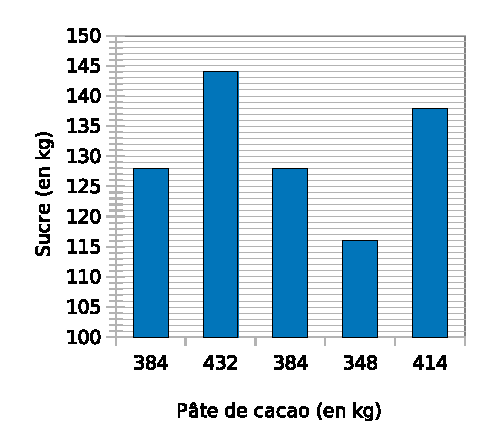
\includegraphics[width=7.7cm]{diag_batons}
\begin{enumerate}
 \item Recopie et complète à l'aide des données du graphique, un tableau comme celui proposé ci‑dessous :
 \vspace{0.5cm}
 \begin{minipage}[c]{0.86\linewidth}
  \begin{tabularx}{\linewidth}{|c|*{4}{>{\centering\arraybackslash}X|}}
  \hline
 \cellcolor{J2} Masse de sucre (en kg) & & & \\\hline
 \cellcolor{J2} Masse de pâte de cacao (en kg) & & & \\\hline
 \end{tabularx}
\end{minipage} \hfill%
 \begin{minipage}[c]{0.1\linewidth}
\vspace{0.5cm}
\ldots

\ldots
\end{minipage} \\
 \item D'après ce tableau, peut‑on dire que la masse de sucre est proportionnelle à celle de la pâte de cacao ? Justifie ta réponse.
 \end{enumerate}
\end{exercice}


\begin{exercice}[Des mélanges]
Une entreprise propose plusieurs types de béton selon la quantité de gravier, de sable et de ciment qu'il comporte.
\begin{center}
 \renewcommand*\tabularxcolumn[1]{>{\centering\arraybackslash}m{#1}}
 \begin{ttableau}{\linewidth}{4}
 \hline
 & \cellcolor{BleuOuv} Gravier & \cellcolor{BleuOuv} Sable & \cellcolor{BleuOuv} Ciment \\\hline
 \cellcolor{BleuOuv} Béton A & 21 kg & 10 kg & 9 kg \\\hline
 \cellcolor{BleuOuv} Béton B & 9 kg & 3,5 kg & 3 kg \\\hline
 \cellcolor{BleuOuv} Béton C & 11 kg & 8,5 kg & 9,5 kg \\\hline
 \end{ttableau}
\end{center}
Parmi ces mélanges, quel est celui qui comporte : 
\begin{enumerate}
 \item La plus grande proportion de gravier ? 
 \item La plus grande proportion de sable ? 
 \item La plus grande proportion de ciment ? 
 \end{enumerate}
Tu justifieras chacune de tes réponses.
\end{exercice}


\begin{exercice}[Diagramme circulaire]
Dans le collège Sésacol, la répartition des élèves en fonction du niveau est la suivante :
\begin{center}
 \begin{tabularx}{\linewidth}{|c|*{4}{>{\centering\arraybackslash}X|}}
  \hline
  \rowcolor{U2} Niveau & 5\up{ème} & 6\up{ème} & 7\up{ème} & 8\up{ème} \\\hline
  \rowcolor{C3} Nombre d'élèves & 126 & 112 & 120 & 122 \\\hline
  \end{tabularx}
 \end{center}
On souhaite représenter ces données à l'aide d'un diagramme circulaire.
\begin{enumerate}
 \item Combien y a‑t‑il d'élèves dans ce collège ? Quelle est la mesure de l'angle au centre d'un secteur angulaire qui représenterait l'ensemble des élèves de ce collège dans un diagramme circulaire ?
 \item Recopie et complète le tableau de proportionnalité suivant :
\vspace{0.3cm}
\begin{center}
 \begin{tabularx}{\linewidth}{|c|*{5}{>{\centering\arraybackslash}X|}}
  \hline
  \rowcolor{U2} Niveau & 6\up{ème} & 5\up{ème} & 4\up{ème} & 3\up{ème} & Total \\\hline
  \rowcolor{C3} Nombre d'élèves & 126 & 112 & 120 & 122 & \\\hline
  \rowcolor{F3} Angle au centre & & & & & $360^\circ$ \\\hline
  \end{tabularx}
 \end{center}
 \vspace{0.3cm}
 \item Trace un cercle de rayon 5 cm et représente la répartition des élèves sous forme de diagramme circulaire.
 \end{enumerate}
\end{exercice}


\end{colonne*exercice}

\connaissances

\QCMautoevaluation{Pour chaque question, plusieurs réponses sont
  proposées.  Déterminer celles qui sont correctes.}

\begin{QCM}
  \begin{GroupeQCM}
    \begin{exercice}
     1 CD coûte 6,50 CHF. Combien coûtent 11 CD ?
      \begin{ChoixQCM}{4}
      \item 65 CHF
      \item 71,5 CHF
      \item 715 CHF
      \item 11 CHF
      \end{ChoixQCM}
\begin{corrige}
     \reponseQCM{b}
   \end{corrige}
    \end{exercice}
    
   
    \begin{exercice}
      1 kg de pommes coûte 1,60 CHF. Rémi paye 1,20 CHF. Il a donc acheté \ldots
      \begin{ChoixQCM}{4}
      \item 750 g de pommes
      \item 0,40 kg de pommes
      \item 1,333 kg de pommes
      \item 0,75 kg de pommes
      \end{ChoixQCM}
\begin{corrige}
     \reponseQCM{ad}
   \end{corrige}
    \end{exercice}
    
    
    \begin{exercice}
      Quelle(s) est (sont) la (les) situation(s) de proportionnalité ?
      \begin{ChoixQCM}{4}
      \item Les dimensions d'une maquette par rapport aux dimensions de l'objet réel.
      \item La taille d'un être humain avec son âge.
      \item La quantité de peinture en fonction de la surface à peindre.
      \item Le prix à payer en fonction du nombre d'articles achetés.
      \end{ChoixQCM}
\begin{corrige}
     \reponseQCM{ac}
   \end{corrige}
    \end{exercice}
    
    
    \begin{exercice}
      Quel(s) est (sont) le (les) tableau(x) de proportionnalité ?
      \begin{ChoixQCM}{4}
      \item
       \begin{tabular}{|c|c|c|}
       \hline
        1 & 2 & 3 \\\hline
        4,5 & 9 & 13,5 \\\hline
        \end{tabular}
      \item
       \begin{tabular}{|c|c|c|}
       \hline
        1 & 2 & 6 \\\hline
        7 & 14 & 41 \\\hline
        \end{tabular}
      \item
       \begin{tabular}{|c|c|c|}
       \hline
        3 & 6 & 9 \\\hline
        7,5 & 15 & 21,5 \\\hline
        \end{tabular}
      \item
       \begin{tabular}{|c|c|c|}
       \hline
        5 & 10 & 20 \\\hline
        9 & 14 & 24 \\\hline
        \end{tabular}
      \end{ChoixQCM}
\begin{corrige}
     \reponseQCM{a}
   \end{corrige}
    \end{exercice}
    
    
    \begin{exercice}
      Si trois baguettes coûtent 2,40 CHF, alors \ldots
      \begin{ChoixQCM}{4}
      \item Cinq baguettes coûtent 4,40 CHF
      \item Dix baguettes coûtent 8 CHF
      \item Six baguettes coûtent 8,20 CHF
      \item Deux baguettes coûtent 1,60 CHF
      \end{ChoixQCM}
\begin{corrige}
     \reponseQCM{bd}
   \end{corrige}
    \end{exercice}
    
    
    \begin{exercice}
      8 fourmis de même taille, en file indienne, mesurent au total 7,2 cm, donc \ldots
      \begin{ChoixQCM}{4}
      \item 7 fourmis   mesurent au total 6,3 cm
      \item 12 fourmis   mesurent au total 10,2 cm
      \item 16 fourmis mesurent au total 144 mm
      \item 2 fourmis mesurent au total 1,6 cm
      \end{ChoixQCM}
\begin{corrige}
     \reponseQCM{ac}
   \end{corrige}
    \end{exercice}
    
    
     \begin{exercice}
      Un nénuphar double de surface tous les jours. En quarante jours, il recouvre un lac.
      \begin{ChoixQCM}{4}
      \item Le lac était recouvert à moitié le vingtième jour
      \item Le quatre‑vingtième jour le nénuphar couvrira deux lacs de même surface
      \item Un quart du lac était recouvert le trente‑huitième jour
      \item La situation présentée est proportionnelle
      \end{ChoixQCM}
\begin{corrige}
     \reponseQCM{c}
   \end{corrige}
    \end{exercice}
    
    
     \begin{exercice}
      Une voiture de course fait un tour de circuit de  14 km en 4 minutes à vitesse constante. Alors \ldots
      \begin{ChoixQCM}{4}
      \item En une heure, elle parcourt 280 km
      \item Elle a parcouru 3,5 km par minute
      \item Elle parcourt en 12 minutes trois fois plus de distance
      \item Elle roule en moyenne à 210 km/h
      \end{ChoixQCM}
\begin{corrige}
     \reponseQCM{bcd}
   \end{corrige}
    \end{exercice}

\end{GroupeQCM}
\end{QCM}

  


\TravauxPratiques % pour nous "travailler en groupe"

\begin{TP}[Le puzzle qui s'agrandit]

\partie{Création d'un modèle}
\begin{minipage}[c]{0.48\linewidth}
\begin{enumerate}
 \item Tracez un carré de 5 cm de côté pour le groupe. Partagez-le en autant de pièces (triangles rectangles, carrés, rectangles, trapèzes \ldots) que de membres du groupe.
 
Vous obtenez un puzzle du carré.
 \item Déterminez ensemble les dimensions de chaque pièce.
 \end{enumerate}
\end{minipage} \hfill%
 \begin{minipage}[c]{0.4\linewidth}
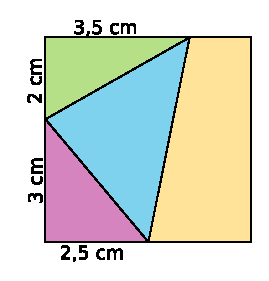
\includegraphics[width=4cm]{carre_puzzle}
 \end{minipage} \\

\partie{Agrandissement}
\begin{enumerate}
 \setcounter{enumi}{2}
 \item On souhaite agrandir le puzzle. \\[0.5em]
Chaque élève du groupe choisit une pièce et la reproduit avec de nouvelles dimensions de façon à ce que le puzzle reconstitué soit un carré de 12 cm de côté.
 \end{enumerate}

\partie{Vérification}
\begin{enumerate}
 \setcounter{enumi}{3}
 \item Vérifiez en essayant de reconstituer le puzzle.
 \end{enumerate}

\end{TP}

%%%%%%%%%%%%%%%%%%%%%%%%%%%%%%%%%%%
%%%%%%%%%%%%%%%%%%%%%%%%%%%%%%%%%%%
%MiseEnPage
%%%%%%%%%%%%%%%%%%%%%%%%%%%%%%%%%%%
\vfill
%%%%%%%%%%%%%%%%%%%%%%%%%%%%%%%%%%%
%%%%%%%%%%%%%%%%%%%%%%%%%%%%%%%%%%%


\pagebreak

\recreation
\begin{enigme}[Les œufs \small{(d’après le GVJM)}]

Deux œufs d’autruche permettent de faire une omelette qu’on pourrait faire avec 45 œufs de poule. Avec 9 œufs de poule, on fait une omelette pour 5 personnes. \\[0.5em]
Combien faudrait-il d’œufs d’autruche pour faire une omelette pour 100 personnes ?

\end{enigme} 

%%%%%%%%%%%%%%%%%%%%%%%%%%%%%%%%%%%%%%%%%%%%%%%%%%%%%%%%%%%%%%%%%%%%%%%%%%

\begin{enigme}[Des billes \small{(source : www.educalire.net)}]

Paul a 20 ans ; il décide de donner ses 738 billes à ses 3 frères, âgés de 11, 14 et 16 ans. Il veut les partager proportionnellement à l’âge de chacun. \\[0.5em]
Combien chaque frère recevra-t-il de billes ?
           
\end{enigme} 

%%%%%%%%%%%%%%%%%%%%%%%%%%%%%%%%%%%%%%%%%%%%%%%%%%%%%%%%%%%%%%%%%%%%%%%%%%

\begin{enigme}[Les pommes \small{(d’après le GVJM)}]

Deux paniers, $A$ et $B$, contiennent des pommes. Il y a 2 fois plus de pommes dans le panier $A$ que dans le panier $B$. Un voleur prend 18 pommes et pourtant il reste encore 2 fois plus de pommes dans le panier $A$ que dans le panier $B$. \\[0.5em]
Combien de pommes ont été volées dans le panier $A$ ?

\end{enigme} 

%%%%%%%%%%%%%%%%%%%%%%%%%%%%%%%%%%%%%%%%%%%%%%%%%%%%%%%%%%%%%%%%%%%%%%%%%%

\begin{enigme}[Les bougies \small{(d’après le GVJM)}]

Fonfon Labricole s’est aperçu que les bougies ne se consument jamais complètement. Avec 7 restes de bougies, il fabrique une grande bougie. \\[0.5em]
Quel est le maximum de grandes bougies qu’il peut allumer avec 49 restes de bougies et un briquet ?

\end{enigme} 

%%%%%%%%%%%%%%%%%%%%%%%%%%%%%%%%%%%%%%%%%%%%%%%%%%%%%%%%%%%%%%%%%%%%%%%%%%


